% uOttawa (unofficial) Thesis Template for LaTeX 
% Edited by Wail Gueaieb based on Stephen Carr's uWaterloo Template

% The files included in this package are slighly modified by Suruz Miah to adapt partial requirements  in writing project/thesis reports of the Bradley University's Department of Electrical and Computer Engineering.

% DON'T USE THIS TEMPLATE IF YOU DON'T KNOW WHAT YOU'RE DOING!
% Remember, it comes WITH NO WARRANTY!

% Please read the "00readme.txt" file first.
% Here is how to use this template:
%
% DON'T FORGET TO ADD YOUR OWN NAME AND TITLE in the "hyperref" package
% configuration in the "thesis-preample.tex" file. THIS INFORMATION GETS 
% EMBEDDED IN THE PDF FINAL PDF DOCUMENT.
% You can view the information if you view Properties of the PDF document.

% The template is based on the standard "book" document class which provides 
% all necessary sectioning structures and allows multi-part theses.

% DISCLAIMER
% To the best of our knowledge, this template satisfies the current 
% uOttawa thesis requirements.
% However, it is your responsibility to assure that you have met all 
% requirements of the university and your particular department.
% Many thanks to the feedback from many graduates that assisted the 
% development of this template.Things

% -----------------------------------------------------------------------

% When using pdflatex, by default the output is geared toward generating a PDF 
% version optimized for viewing on an electronic display, including 
% hyperlinks within the PDF.
 
% E.g. to process a thesis based on this template, run:

% (pdf)latex thesisMain	-- first pass of the (pdf)latex processor
% bibtex thesisMain 	-- generates bibliography from .bib data file(s) 
% (pdf)latex thesisMain	-- fixes cross-references, bibliographic references, etc
% (pdf)latex thesisMain	-- fixes cross-references, bibliographic references, etc
% makeindex -s nomentbl.ist -o thesisMain.nls thesisMain.nlo
% (pdf)latex thesisMain	-- fixes cross-references, bibliographic references, etc
% (pdf)latex thesisMain	-- fixes cross-references, bibliographic references, etc



% N.B. The "pdftex" program allows graphics in the following formats to be
% included with the "\includegraphics" command: PNG, PDF, JPEG, TIFF
% Tip 1: Generate your figures and photos in the size you want them to appear
% in your thesis, rather than scaling them with \includegraphics options.
% Tip 2: Any drawings you do should be in scalable vector graphic formats:
% SVG, PNG, WMF, EPS and then converted to PNG or PDF, so they are scalable in
% the final PDF as well.
% Tip 3: Photographs should be cropped and compressed so as not to be too large.

% To create a PDF output that is optimized for double-sided printing: 
%
% 1) comment-out the \documentclass statement in the preamble below, and
% un-comment the second \documentclass line.
%
% 2) change the value assigned below to the boolean variable
% "PrintVersion" from "false" to "true".

% --------------------- Start of Document Preamble -----------------------

% Specify the document class, default style attributes, and page dimensions
% For hyperlinked PDF, suitable for viewing on a computer, use this:
\documentclass[letterpaper,12pt,titlepage,oneside,final]{book}
 
% For PDF, suitable for double-sided printing, change the PrintVersion variable below
% to "true" and use this \documentclass line instead of the one above:
% \documentclass[letterpaper,12pt,titlepage,openright,twoside,final]{book}


% This package allows if-then-else control structures.
\usepackage{ifthen}
\newboolean{PrintVersion}
\setboolean{PrintVersion}{false} 
% \setboolean{PrintVersion}{true} 
% CHANGE THIS VALUE TO "true" as necessary, to improve printed results 
% for hard copies by overriding some options of the hyperref package.


% Load your needed packages and other commands of yours.
% Load your needed packages and other commands of yours here:
%\usepackage{} % ... note that old .sty files can be included here

%--------------------------------------------------------------------------
% Do NOT edit the rest of the preample UNLESS YOU KNOW WHAT YOU'RE DOING!
%--------------------------------------------------------------------------

\ifthenelse{\boolean{PrintVersion}}{
\usepackage[top=1in,bottom=1in,left=0.75in,right=1.25in]{geometry}   % For twoside document
}{
\usepackage[top=1in,bottom=1in,left=0.75in,right=1.25in]{geometry}   % For oneside document
}

\usepackage{amsmath,amssymb,amstext} % Lots of math symbols and environments
\usepackage{graphicx} % For including graphics 

\usepackage{nomentbl} 
\makenomenclature 

\usepackage{ifpdf}

\newcommand{\href}[1]{#1} % does nothing, but defines the command so the
    % print-optimized version will ignore \href tags (redefined by hyperref pkg).
%\newcommand{\texorpdfstring}[2]{#1} % does nothing, but defines the command
% Anything defined here may be redefined by packages added below...


% Hyperlinks make it very easy to navigate an electronic document.
% In addition, this is where you should specify the thesis title
% and author as they appear in the properties of the PDF document.
% Use the "hyperref" package 
% N.B. HYPERREF MUST BE THE LAST PACKAGE LOADED; ADD ADDITIONAL PKGS ABOVE
\usepackage[\ifpdf pdftex,\fi letterpaper=true,pagebackref=false]{hyperref} % with basic options
		% N.B. pagebackref=true provides links back from the References to the body text. This can cause trouble for printing.
\hypersetup{
    plainpages=false,       % needed if Roman numbers in frontpages
    pdfpagelabels=true,     % adds page number as label in Acrobat's page count
    bookmarks=true,         % show bookmarks bar?
    unicode=false,          % non-Latin characters in Acrobat's bookmarks
    pdftoolbar=true,        % show Acrobat's toolbar?
    pdfmenubar=true,        % show Acrobat's menu?
    pdffitwindow=false,     % window fit to page when opened
%    pdftitle={uOttawa\ LaTeX\ Thesis\ Template},    % title: CHANGE THIS TEXT!
%    pdfauthor={Author},    % author: CHANGE THIS TEXT! and uncomment this line
%    pdfsubject={Subject},  % subject: CHANGE THIS TEXT! and uncomment this line
%    pdfkeywords={keyword1} {key2} {key3}, % list of keywords, and uncomment this line if desired
    pdfnewwindow=true,      % links in new window
    colorlinks=true,        % false: boxed links; true: colored links
    linkcolor=blue,         % color of internal links
    citecolor=green,        % color of links to bibliography
    filecolor=magenta,      % color of file links
    urlcolor=blue           % color of external links
}
\ifthenelse{\boolean{PrintVersion}}{   % for improved print quality, change some hyperref options
\hypersetup{	% override some previously defined hyperref options
%    colorlinks,%
    citecolor=black,%
    filecolor=black,%
    linkcolor=black,%
    urlcolor=black}
}{} % end of ifthenelse (no else)

\usepackage{fancyhdr,lastpage} % Change caption style; changes headers and page styles etc.

\usepackage{subfigure}
\usepackage{subfloat}
\usepackage{epstopdf}
\epstopdfsetup{suffix = {}}
\usepackage{float}
\usepackage{graphicx}
\usepackage{algorithm}              % Used for the pseudocode section
\usepackage[noend]{algpseudocode}   % Used for the pseudocode section

\usepackage{enumerate}
\usepackage{siunitx}
\sisetup{unitsep=\cdot}
\usepackage{booktabs}
%\usepackage{nohyperref}
\usepackage{tikz}
\usetikzlibrary{calc}
\def\myGrid{0.5}
\usepackage{todonotes}
\usepackage[english,algo2e,algoruled,vlined,linesnumbered]{algorithm2e}   % package for algorithm
\usepackage{soul}
\usepackage{xtab}
\usepackage[perpage,para,symbol*]{footmisc}




% This is where thesis margins and spaces are set.
% Setting up the page margins...
% A minimum of 1 inch (72pt) margin at the
% top, bottom, and outside page edges and a 1.125 in. (81pt) gutter
% margin (on binding side). While this is not an issue for electronic
% viewing, a PDF may be printed, and so we have the same page layout for
% both printed and electronic versions, we leave the gutter margin in.
% Set margins:
\setlength{\marginparwidth}{0pt} % width of margin notes
% N.B. If margin notes are used, you must adjust \textwidth, \marginparwidth
% and \marginparsep so that the space left between the margin notes and page
% edge is less than 15 mm (0.6 in.)
\setlength{\marginparsep}{0pt} % width of space between body text and margin notes
\setlength{\evensidemargin}{0.125in} % Adds 1/8 in. to binding side of all 
% even-numbered pages when the "twoside" printing option is selected
\setlength{\oddsidemargin}{0.125in} % Adds 1/8 in. to the left of all pages
% when "oneside" printing is selected, and to the left of all odd-numbered
% pages when "twoside" printing is selected
\setlength{\textwidth}{6.375in} % assuming US letter paper (8.5 in. x 11 in.) and 
% side margins as above
\raggedbottom

% The following statement specifies the amount of space between
% paragraphs. Other reasonable specifications are \bigskipamount and \smallskipamount.
\setlength{\parskip}{\medskipamount}

% The following statement controls the line spacing.  The default
% spacing corresponds to good typographic conventions and only slight
% changes (e.g., perhaps "1.2"), if any, should be made.
\renewcommand{\baselinestretch}{1} % this is the default line space setting

% By default, each chapter will start on a recto (right-hand side)
% page.  We also force each section of the front pages to start on 
% a recto page by inserting \cleardoublepage commands.
% In many cases, this will require that the verso page be
% blank and, while it should be counted, a page number should not be
% printed.  The following statements ensure a page number is not
% printed on an otherwise blank verso page.
\let\origdoublepage\cleardoublepage
\newcommand{\clearemptydoublepage}{%
  \clearpage{\pagestyle{empty}\origdoublepage}}
\let\cleardoublepage\clearemptydoublepage



\fancypagestyle{myFancy}{%
  \fancyhf{}% Clear header and footer
  \fancyhead[LE,RO]{\bfseries\nouppercase{\rightmark}}
  \fancyhead[LO,RE]{\bfseries\nouppercase{\leftmark}}
  \fancyfoot[R]{Page \thepage\ of \pageref{LastPage}}% Custom footer
  \fancyfoot[L]{E.~Jones, D.~Adra,~S.~Miah}% Custom footer
  \renewcommand{\headrulewidth}{0.4pt}% Line at the header visible
  \renewcommand{\footrulewidth}{0.1pt}% Line at the footer visible
}


%======================================================================
%   L O G I C A L    D O C U M E N T -- the content of your thesis
%======================================================================
\begin{document}

% For a large document, it is a good idea to divide your thesis
% into several files, each one containing one chapter.
% To illustrate this idea, the "front pages" (i.e., title page,
% declaration, borrowers' page, abstract, acknowledgements,
% dedication, table of contents, list of tables, list of figures,
% nomenclature).
%----------------------------------------------------------------------
% FRONT MATERIAL
%----------------------------------------------------------------------
%
% C O V E R  P A G E
% ------------------
\newcommand{\thesisauthor}{Dakota Adra and Eric Jones}
\newcommand{\advisor}{Dr. Suruz Miah}
\newcommand{\thesistitlecoverpage}{%
Area Coverage Optimization 
}
%\newcommand{\degree}{Ph.D.} % possible values are:
                            % M.A. / M.A.Sc. / M.Sc. / MCS / Ph.D.
\newcommand{\nameofprogram}{Electrical and Computer Engineering Department}
\newcommand{\academicunit}{Caterpillar College of Engineering and Technology}
%\newcommand{\faculty}{Faculty of Engineering}
\newcommand{\nameOfUniversity}{Bradley University}
\newcommand{\graduationyear}{2019}
%
% T I T L E   P A G E
% -------------------
% Last updated May 24, 2011, by Stephen Carr, IST-Client Services
% The title page is counted as page `i' but we need to suppress the
% page number.  We also don't want any headers or footers.
\pagestyle{empty}
\pagenumbering{roman}

% The contents of the title page are specified in the "titlepage"
% environment.
\begin{titlepage}
        \begin{center}
        \vspace*{1.0cm}

        \Huge
        {\bf \thesistitlecoverpage }

        \vspace*{1.0cm}

        \normalsize
        by \\

        \vspace*{1.0cm}

        \Large
        \thesisauthor\\
        Advisor:~\href{http://personalpages.bradley.edu/~smiah/}{\advisor}\\

        \vspace*{3.0cm}

        % \normalsize
        % Thesis submitted to the\\
        % Faculty of Graduate and Postdoctoral Studies\\
        % In partial fulfillment of the requirements\\
        % For the \degree~degree in\\
        % \nameofprogram\\

        \vspace*{2.0cm}

        \nameofprogram\\
        \academicunit\\
        %\faculty\\
        \nameOfUniversity\\

        \vspace*{4.0cm}

        \copyright~\thesisauthor, Peoria, Illinois, \graduationyear\\
        \end{center}
\end{titlepage}

% The rest of the front pages should contain no headers and be numbered using Roman numerals starting with `ii'
% PRELIMINARY PAGES

\pagestyle{plain}
\setcounter{page}{2}

\cleardoublepage % Ends the current page and causes all figures and tables that have so far appeared in the input to be printed.
% In a two-sided printing style, it also makes the next page a right-hand (odd-numbered) page, producing a blank page if necessary.



%%% Local Variables:
%%% mode: latex
%%% TeX-master: "../thesisMain"
%%% End:




%
% R E S T  O F  F R O N T  P A G E S
% ----------------------------------
% % D E C L A R A T I O N   P A G E
% -------------------------------
  % This page is not needed for a uOttawa thesis. Don't include it.
  % It is designed for an electronic thesis.
  \noindent
I hereby declare that I am the sole author of this thesis. This is a true copy of the thesis, including any required final revisions, as accepted by my examiners.

  \bigskip
  
  \noindent
I understand that my thesis may be made electronically available to the public.

\cleardoublepage
%\newpage
 %This is not needed in a uOttawa thesis.
%
% Edit the following 3 files with your abstract, acknowledgements, 
% and dedication.
% A B S T R A C T
% ---------------

\begin{center}\textbf{Abstract}\end{center}

The project implements an area coverage optimization algorithm using a cost-effective and open-source platform of multiple autonomous robots. The cost-effective ad open-source platform developed in this work is Multi-Agent Framework Open-Source Software (MAFOSS). A team of mobile robots are deployed in a spatial area in a manner so that the asymptotic configurations of robots in the area  yields its maximum coverage. A scalar field, called herein the density, is used to define the coverage metric of the area where the robots are deployed. A large body of research has been conducted in the literature to date for solving such area coverage optimization problems. However, most of the algorithms are either tested in simulations are implemented using a particular set of robotic platforms, which are commercially available for limited operations. In this project, we generalize the implementation platform using the proposed MAFOSS system, where a team of mobile robots is not only employed for developing an area coverage algorithm but also for developing a set of motion control algorithms using multiple autonomous homogeneous/heterogeneous robots operating in a two-dimensional area. The proposed implementation platform is tested in a commercially available simulation platform, Virtual Robot Experimentation Platform (V-REP) in cooperation with robot operating system (ROS).  In addition, a set of experiments using multiple open-source robotic platforms, EduMODs, in cooperation with ROS has been conducted to demonstrate the effectiveness of the proposed platform, MAFOSS.   


\cleardoublepage
%\newpage


%%% Local Variables:
%%% mode: latex
%%% TeX-master: "../finalReportMainV1"
%%% End:

% A C K N O W L E D G E M E N T S
% -------------------------------

\begin{center}\textbf{Acknowledgements}\end{center}

I would like to thank all the little people who made this possible.


\cleardoublepage
%\newpage



%%% Local Variables:
%%% mode: latex
%%% TeX-master: "../finalReportMainV1"
%%% End:

% % D E D I C A T I O N
% -------------------

\begin{center}\textbf{Dedication}\end{center}

This is dedicated to the one I love.


\cleardoublepage
%\newpage


%%% Local Variables:
%%% mode: latex
%%% TeX-master: "../finalReportMainV1"
%%% End:

%
%
% No need to edit this file.
% T A B L E   O F   C O N T E N T S
% ---------------------------------
\renewcommand\contentsname{Table of Contents}
\tableofcontents
\cleardoublepage
\phantomsection
%\newpage

% L I S T   O F   T A B L E S
% ---------------------------
\addcontentsline{toc}{chapter}{List of Tables}
\listoftables
\cleardoublepage
\phantomsection		% allows hyperref to link to the correct page
%\newpage

% L I S T   O F   F I G U R E S
% -----------------------------
\addcontentsline{toc}{chapter}{List of Figures}
\listoffigures
\cleardoublepage
\phantomsection		% allows hyperref to link to the correct page
%\newpage


%
% No need to edit this file. But you may want to comment the whole line if you
% don't have or want a Nomenclature section.
% L I S T   O F   S Y M B O L S
% -----------------------------
% To include a Nomenclature section
\addcontentsline{toc}{chapter}{\textbf{Nomenclature}}

\renewcommand{\nomname}{Nomenclature}
\renewcommand{\nomAname}{\textbf{\large Abbreviations}}
\renewcommand{\nomGname}{\textbf{\large Mathematical Symbols}}
\renewcommand{\nomXname}{\textbf{\large Superscripts}}
\renewcommand{\nomZname}{\textbf{\large Subscripts}}

\printnomenclature
\cleardoublepage
\phantomsection % allows hyperref to link to the correct page
% \newpage


\nomAname
\bigbreak
\textbf{EduMOD}  $\ldots\ldots\ldots\ldots\ldots$

\textbf{MAFOSS}  Multi-agent framework open--source software 

\textbf{Pose}  Position and orientation

\textbf{ROS}  Robot Operating System


%%% Local Variables: 
%%% mode: latex
%%% TeX-master: "../uottawa-thesis"
%%% End:   


% Change page numbering back to Arabic numerals
\pagenumbering{arabic}



%

% Redefine the plain page style
\fancypagestyle{plain}{%
  \fancyhf{}%
  \fancyfoot[R]{Page \thepage\ of \pageref{LastPage}}%
  \fancyfoot[L]{E.~Jones, D.~Adra,~S.~Miah}%  
  \renewcommand{\headrulewidth}{0pt}% Line at the header invisible
  \renewcommand{\footrulewidth}{0.1pt}% Line at the footer visible
}

\pagestyle{myFancy}


%----------------------------------------------------------------------
% MAIN BODY
%---------------------------------------------------------------------- 
% Chapters 
% Include your "sub" source files here (must have extension .tex)
%======================================================================
\chapter{Introduction}
\label{sec:introductionAreaCoverageOptimization}
%======================================================================


\section{Background Study} %review of literature and prior work
%========================================================================================
%   BACKGROUND STUDY   %
%========================================================================================
Many papers have been published on algorithms requiring multi\-agent systems to optimize area coverage. However, few of these works describe a flexible framework that provides the means to achieve such a coverage task. 

Authors in~\cite{Kilinc2015} Kilinic attempts to optimize area coverage of an interconnected network of sensors and actuators that act as a control system. Kilinic’s goal is to maximize the area coverage of the wireless network control system (WNCS) whilst still maintaining convergence of the system in a large environment. Possible applications for the such a control system include smart grid, automatic management and navigation systems.  

The system is arranged in several heterogeneous subnetworks that communicate ad-hoc.  A single packet of information will hop multiple times through the network until it reaches the Kalman filter. Each of the subnetworks has a connection to the Kalman filter whilst remaining separate from each other. The Kalman filter is used to account for asymmetric packet arrival times as well as packet loss.  

In \cite{Lee2015} Lee attempts to optimize the area of a given region of interest for a time variant density. Dynamic density coverage has additional application compared to static density coverage. An example of this additional utility can be seen in a search and rescue scenario where the probability of a missing person being found in a particular area is time variant. 

Lee’s algorithm works by using voronoi regions and a robotic cost function to determine area coverage. Each robot is responsible for covering a particular voronoi region. Time information is used in the robot movement to account for the rapid changes in the density functions. 

In \cite{Miah2018} Miah adapts previous attempts of area coverage by using a fleet of heterogeneous modular cost-effective robots in real time. This allows for heterogeneous or non-uniform resource allocation and stabilizes the algorithm to allow for variation in the abilities of the constituent robots. 

The algorithm in Miah’s research is very similar to that of Lee’s. Miah adds additional consideration for the robot actuation limitations for a heterogeneous case whilst Lee does not. Each individual robot is given a coverage metric to describe its area coverage performance. 

In “Sensing and coverage for a network of heterogeneous robots” \cite{Pimenta2009} Pimenta is attempting to adapt the area coverage model for intruder tracking. Multiple intruders in a specified region can be tracked using this method even if their location is unknown. The coverage is optimized and therefore the probability or detecting any existing intruders in the area is also maximized.  

Pimenta’s algorithm allows an individual robot to track an intruder in its Voronoi cell whilst the other robots respond to provide optimal area coverage. When an intruder is located within a given distance from a robot it will trigger that particular robot to follow the intruder. 

In \cite{Varposhti2016} Varposhti uses area coverage optimization to distribute mobile directional sensors over an area. The sensors can move around freely and can adapt in the case of an outage in a particular area. Such networks can be used in target tracking, search and rescue, and surveillance. 

Varposhti uses a distributed learning algorithm to achieve area coverage in his research. Each sensor collaborates with its neighbors to determine the best position and orientation for each sensor. Each sensor moves in a random direction and turns in a random position until the coverage is maximized. 

In \cite{Yu2018} Yu attempts to find the optimal area coverage for deployable reconnaissance sensors. His approach involves considering the areas in which the sensors can be deployed, the connectivity and the coverage. Such an algorithm provides the ability to deploy sensors almost anywhere for the purpose of surveillance and intelligence. 

Yu’s algorithm uses genetic neural networks and particle swarm optimization to achieve optimal deployment. In the genetic algorithm the best performing configurations are passed on to the next generation whilst the poorly performing configurations are slowly phased out. Additionally a mutation rate is maintained to allow for other behavior that was not previously available in an older generation. 

  


%%% Local Variables:
%%% mode: latex
%%% TeX-master: "../finalReportMainV1"
%%% End:

\chapter{Modeling Area Coverage Optimization}
\label{chap:areaCoverageModeling}

\section{Introduction}
\label{sec:introAreaCoverageModeling}

\section{Conclusion}
\label{sec:conclusionAreaCoverageModeling}
% Some LaTeX commands I define for my own nomenclature.
% If you have to, it's better to change nomenclature once here than in a 
% million places throughout your thesis!
\newcommand{\package}[1]{\textbf{#1}} % package names in bold text
\newcommand{\cmmd}[1]{\textbackslash\texttt{#1}} % command name in tt font 


%======================================================================
\chapter{MAFOSS}
\label{chap:MAFOSS}
%======================================================================


\section{Introduction}
\label{sec:introductionMAFOSS}
This chapter presents a new multi-agent framework using open-source software (MAFOSS). The proposed framework is a modular and cost-effective open-source hardware and software platform that is intended to help develop multi-agent systems for research and education.  Numerous multi-agent platforms have been developed in the literature to date that are used in various robotic applications, such as surveillance, target localization, cooperative estimation, among others. However, most of them are either tailored towards particular applications or driven by expensive software and hardware. The proposed MAFOSS system is developed for robotic applications, where a team of mobile agents (robots) is deployed to achieve a common goal. The software architecture of the current framework mostly relies on robot operating system (ROS). Regardless of internal hardware and/or software architecture, appropriate actions can be applied to actuators of an individual or a team of mobile agents for controlling their motions. A few case studies have been conducted to evaluate the performance of MAFOSS.


The development of multi-agent systems has been of crucial importance in modern autonomous agent-based applications, such as area coverage~\cite{Cortes2004,Lekien2009,MiNgBoSp2014-j1}, perimeter surveillance and environment monitoring~\cite{Pimenta2013,Zhang2013,Rossi2016},  cooperative estimation and formation control~\cite{Spinello2014,Marshall2004,Ge2017,Li2017}, indoor navigation~\cite{GuMi2008-j1,KnHeMi2017-c1} using mobile robots, among others. Typical problems in such applications are usually solved using an array of networked mobile agents operating collectively. Recently, the implementation of various algorithms has been restricted to a fleet of homogeneous robots at high monetary cost. The purpose of this research is to lower the costs of entry due to the selected robot platform by providing an easily accessible framework for heterogeneous robots that can be implemented both expediently and efficiently. Note that the terms robot and agent will be used interchangeably from now on.  While the performance of the most promising multi-agent control algorithms proposed in the literature is evaluated using computer simulations only, a few multi-agent control algorithms have been validated using experiments that fit for particular implementation platforms (\textit{i.e.,} use of specific robots, for example). See the work performed by authors in~\cite{Marshall2004,MiKn2018-j1,MiKnHe2018-j1}, for instance. Therefore, this paper aims to develop an open hardware/software architecture, MAFOSS, to implement multi-agent control algorithms. Two case studies have been implemented using MAFOSS. Some of the major advantages of the MAFOSS include its scalability, low cost, robustness, and open source nature. These qualities enable users to develop algorithms on a larger scale than was previously possible. 
%
The open source environment brings a wide range of support whilst maintaining a fast moving and non-proprietary code base. There are many packages in ROS that allow a user to interface sensors, actuators, and other hardware directly into their system with minimal development required. As such, it is an excellent tool for anyone looking to expand or help standardize their implementation of different algorithms in the fields of cooperative estimation and navigation. 



\section{Overall MAFOSS Architecture}
\label{sec:overallArchitecture}
The overall architecture of the proposed MAFOSS is shown in  Fig.~\ref{fig:MAFOSS-OverallArchitecture}. %
%
\begin{figure}
  \centering
  \fcolorbox{blue}{gray!5}{
    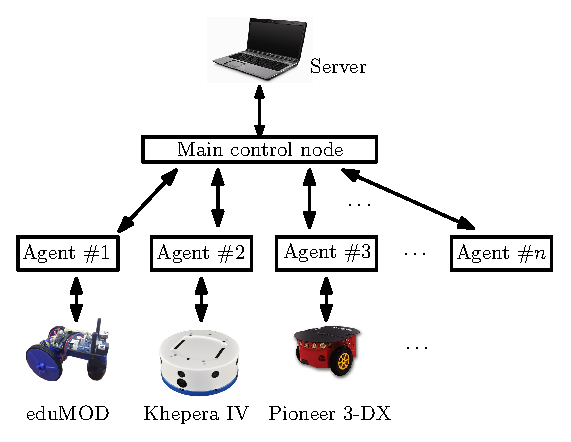
\includegraphics[width=0.45\textwidth]{figs/ipe/networkingOutline.eps}
  }
    \caption{Overall architecture of MAFOSS.}
    \label{fig:MAFOSS-OverallArchitecture}
\end{figure}
%
Therein, $n$ (mobile) agents and the main control node are connected through a local or wide area network used in the proposed framework. After the network has been configured, a multi-agent algorithm can be implemented in the central node. Using this algorithm, the actuator commands determined by the central node are sent to all agents for appropriate actions. The agents collect the measurements and pass relevant data back to the central node as well as prepare to receive new data. All the agent platforms are running ROS, an open source robotics operating system. The client software installed in the central node depends on a particular application within a multi-agent systems. For example, the authors of this paper have documented two case studies where MATLAB's Robot System Toolbox\footnote{https://www.mathworks.com/products/robotics.html} was used as the client software. Note that MATLAB is not open-source, however the decision to use MATLAB was done to save time in the implementation process.  

As a proof of concept, let us consider an area coverage problem~\cite{MiKn2018-j1,MiFaSp2017-j1,MiPaFaSp2017-j1,MiNgBoSp2015-j1}, where a group of mobile autonomous agents are deployed in an area of interest. The problem is to deploy a group of mobile agents such that the coverage metric is maximized. In this case, the central node of the proposed MAFOSS architecture is assigned to implement the area coverage algorithm. For that, appropriate actuator commands for each mobile agent are dispatched at a regular time intervals. The details on how these area coverage algorithms work can be sought in~\cite{MiKn2018-j1,MiFaSp2017-j1,MiPaFaSp2017-j1,MiNgBoSp2015-j1}.  The next section illustrates the software architecture of the MAFOSS that can be used to implement a set of algorithms that use autonomous agents for solving problems of multi-agent systems.
  

%================================================================================================
%================================================================================================
\section{Software Architecture}
\label{sec:softwareArch}
Fig~\ref{fig:MafossSoftwareArchitecture} shows the higher-level software architecture of the proposed MAFOSS. %
%
\begin{figure}
  \centering
              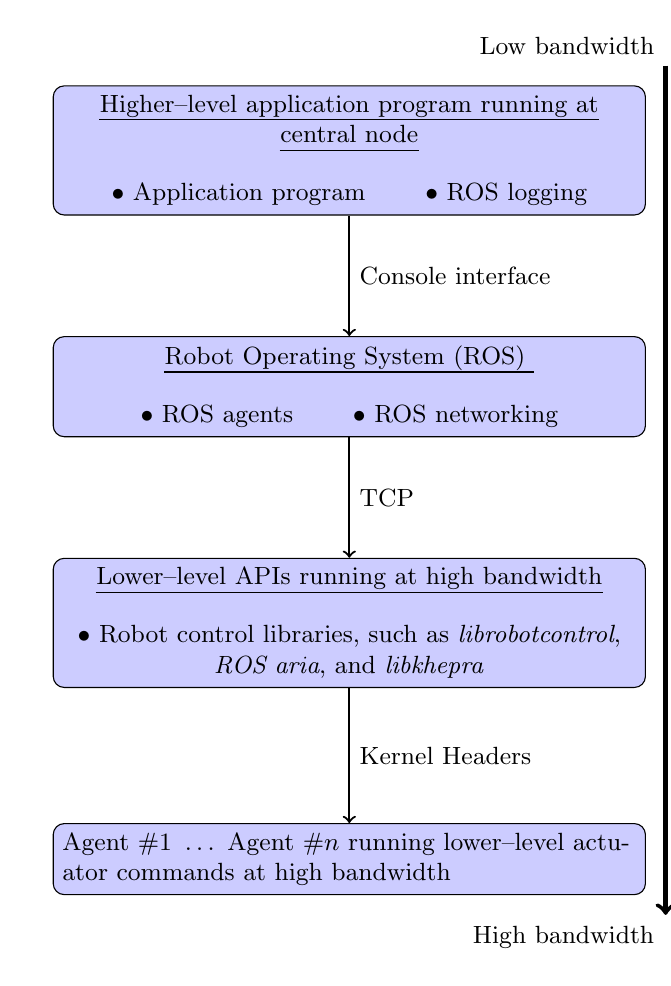
\begin{tikzpicture}
                \tikzstyle{every node} = [font =\small]
                % \tikzstyle{block} = [draw, fill=blue!20, rectangle, 
                % minimum height=3em, minimum width=6em]
                \tikzstyle{block} = [draw, fill=blue!20, rectangle, rounded corners]      
                \tikzstyle{pinstyle} = [pin edge={to-,thin,black}]
                % 
                % 
                \node [block,text width=0.45\textwidth] (userApplication) { \centering \ul{Higher--level application program running at central node}\\
                  \begin{center}
                    $\bullet$~Application program \qquad$\bullet$ ROS logging
                  \end{center}  
                };
                \node[block, text width=0.45\textwidth, below of =userApplication, node distance=3.0cm](ROS){
                  \centering 
                  \ul{Robot Operating System (ROS) }\\
                  \begin{center}
                    $\bullet$~ROS agents \qquad$\bullet$ ROS networking
                  \end{center}
                  };                    
                \node[block, text width=0.45\textwidth, below of =ROS, node distance=3.0cm](controlAPI){
                  \centering 
                  \ul{Lower--level APIs running at high bandwidth}\\
                  \begin{center}
                    $\bullet$~Robot control libraries, such as \emph{librobotcontrol}, \emph{ROS aria}, and \emph{libkhepra}
                  \end{center}
                };
                \node[block, text width=0.45\textwidth, below of =controlAPI, node distance=3.0cm](agents){
                  \centering 
                  $\text{Agent}~\#1~\ldots~\text{Agent}~\#n$ running lower--level actuator commands at high bandwidth
                  };                                 
                % \node[block, text width=1.5cm, right of =inSignalConditioning, node distance=3.5cm](ADC){\emph{BBBlue's 12-bit ADC}};                
                % Draw arrows
                  \draw[->,thick] (userApplication) -- node[midway,right]{Console interface}  (ROS);
                  \draw[->,thick] (ROS) -- node[midway,right]{TCP}  (controlAPI);
                  \draw[->,thick] (controlAPI) -- node[midway,right]{Kernel Headers}(agents);
                  \draw[->,ultra thick]($(userApplication.north east) + (0.5*\myGrid,0.5*\myGrid)$)node[above left]{Low bandwidth} --($(agents.south east) + (0.5*\myGrid,-0.5*\myGrid)$)node[below left]{High bandwidth};
              \end{tikzpicture}  
  \caption{High-level software architecture of MAFOSS.}
  \label{fig:MafossSoftwareArchitecture}
\end{figure}
%
The software architecture is divided into four layers. Each layer executes a set of APIs and dispatches the output to the next layer. The higher-level commands are executed at the central node. Therefore, the bandwidth of operations generated by the algorithm running at the main control node is low. The low-level actuator commands that are run on each agent are executed at high-bandwidth. A detailed description of each layer of the software architecture is provided below. %
%

Fig.~\ref{fig:MAFOSS-OverallArchitecture} details three different robots that act as MAFOSS agents. From left to right there is the eduMOD robot, the Khepera IV robot designed by K-TEAM\footnote{https://www.k-team.com/}, and the Pioneer P3-DX designed by Pioneer Robotics\footnote{https://www.pioneer-robotics.no/}. The eduMOD robot is based on the eduMiP project developed by University of California San Diego's Flow Control and Coordinated Robotics Lab\footnote{https://www.ucsdrobotics.org/}. This robot has been modified into a tricycle configuration (hence the name \emph{eduMOD}), due to the author's desire to improve the accuracy and consistency of its movement. The eduMOD's low-level control APIs and front caster assemblage were designed and developed by the authors of this paper. The eduMOD was created to act as a low-cost, easy to use, and powerful alternative to the large variety of similar tricycle configuration differential-drive mobile robotic platforms.
%
\begin{itemize}
    \item \textbf{Higher-level application program} - The high-level application program in the MAFOSS takes user input, such as agents' initial poses (positions and orientations), alongside workspace parameters, and feeds them into a server that implements multi-agent algorithms. This server communicates to the \emph{Main control node} and forwards this information through ROS to the rest of the system. 
    %========================================================================================
    \item \textbf{Robot Operating System} - The Robotic Operating System (ROS) is a flexible framework for writing robot software. It is a collection of tools, libraries, and conventions that aim to simplify the task of creating complex and robust robot behavior across a wide variety of robotic platforms. In the current MAFOSS, it uses the networking abilities of ROS to define individual agents as nodes to standardize the way a user can approach the algorithm's implementation.  
    %========================================================================================
    \item \textbf{Lower-level APIs} - The lower--level control APIs in this architecture are each dependent on the target agent/robot the user is attempting to interface with. For an embedded computer, such as Beaglebone Blue\footnote{https://beagleboard.org/blue}, the authors use the well-documented robot control library, \emph{librobotcontrol}, as it is specifically intended to be implemented on the Beaglebone. For the Khepera and the Pioneer, the authors will be using the proprietary interfacing firmware developed by their respective companies: the ROS Aria library and libkhepera. The direct hardware interfacing will be done through the Linux Headers, as described in each API.
      % ========================================================================================
    \item \textbf{Agents} - Here are the agents that are interfaced with via the Control APIs as seen in Fig.~\ref{fig:MAFOSS-OverallArchitecture}. These agents are controlled via low-level control code that is present as part of the firmware of each robot or as developed by the user in the case of the eduMOD.
\end{itemize}

To summarize, the software architecture consists of a High level application, the Robotics Operating System, Low-level High bandwidth APIs and the Agents themselves. In general the high level applications consist of user defined behaviors that determine the usage scenario for the MAFOSS architecture. Next, ROS is used for its networking abilities and flexibility when handling a variety of hardware configurations. The Lower level APIs are used to interface directly with the hardware prior to receiving command from ROS. Finally, the Agents themselves are designated by the end user to accomplish the desired task. 


\section{MAFOSS Networking Setup}
\label{sec:networking}
The purpose of this section is to highlight the setup of the network architecture of the MAFOSS. There are various ways to ship data around a network, and each has advantages and disadvantages, depending largely on the application. The communication protocol, such as  transmission control protocol (TCP)  is widely used because it provides a simple and reliable communication stream. TCP packets always arrive in order and lost packets are resent from source to destination until they arrive (see~\cite[Ch.~3]{Kurose2017} for details).

Fig.~\ref{fig:rosNetworkingExample} gives a holistic view on the networking within the MAFOSS using ROS\footnote{http://wiki.ros.org/ROS/Concepts}. Note that the ports specified to the TCP/IP sockets in the \emph{Example} section are arbitrary. Further, the full URI for the master node will include the standard $11311$ port in ROS. %
%
\begin{figure}
    \centering
    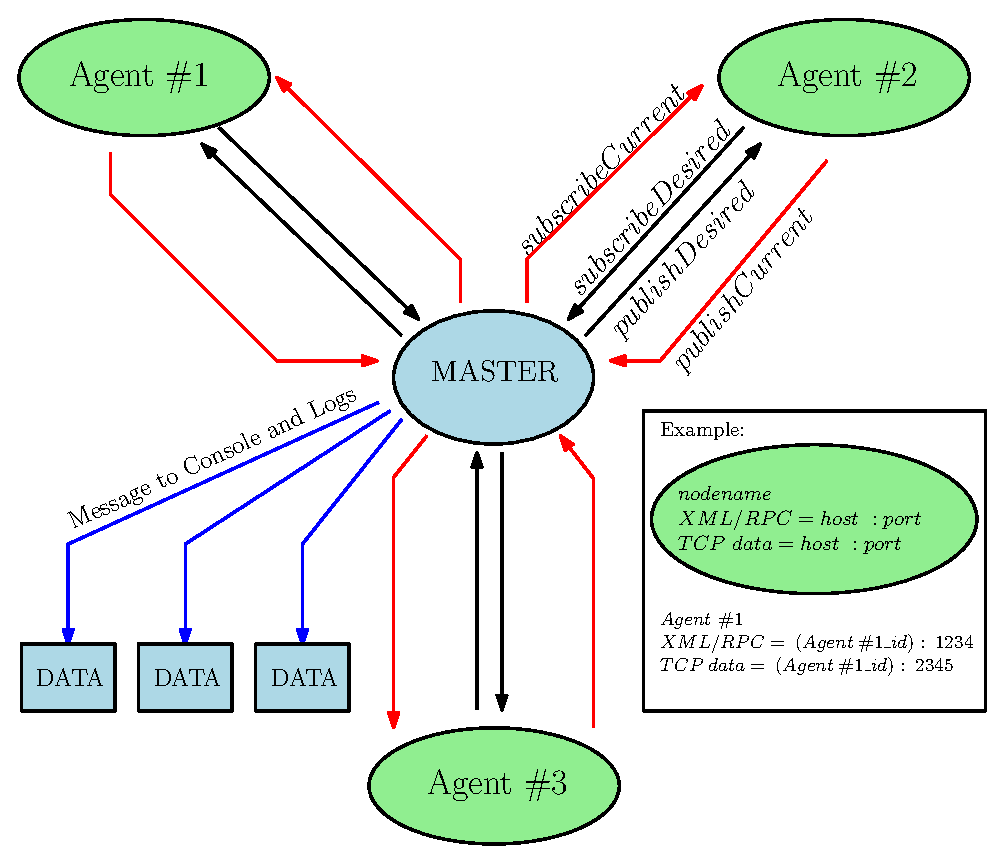
\includegraphics[width=0.48\textwidth]{figs/ipe/rosNetworkingExampleV2.eps}
    \caption{ROS networking.}
    \label{fig:rosNetworkingExample}
  \end{figure}
%  
%========================================================================================
\begin{itemize}
    \item \textbf{Nodes} - Nodes are executables that use ROS to communicate to other nodes through TCPROS across a corresponding \emph{Topic}. In Fig.~\ref{fig:rosNetworkingExample}, the nodes in question are \emph{Agent \#1}, \emph{Agent \#2}, and \emph{Agent \#3}.
    %========================================================================================
    \item \textbf{Topics} - Topics are named buses over which nodes exchange messages. In general, nodes are not aware of who they are communicating with. Instead, nodes that are interested in data \emph{subscribe} to the relevant topic; nodes that generate data \emph{publish} to the relevant topic. Fig.~\ref{fig:rosNetworkingExample} lists four topics associated with the MAFOSS networking as \emph{subscribeCurrent}, \emph{subscribeDesired}, \emph{publishCurrent}, and \emph{publishDesired}. Each node communicating with the MASTER in the MAFOSS system will get its own set of four topics with further designation between each node. For Agent~$\#1,$ the full topic name would be \emph{agent\#1PublishDesired}: this convention will be carried throughout the system independent of the number of agents. %========================================================================================
    \item \textbf{Master} - The ROS Master provides naming and registration services to the rest of the nodes in the ROS system. It tracks publishers and subscribers to topics. The role of the Master is to enable individual ROS nodes to locate one another. Once these nodes have located each other they will begin to communicate with each other peer-to-peer. 
    %========================================================================================
    \item \textbf{Output data} - Output data in the MAFOSS is sent to the main control node and computer running the master node as the raw x and y positions. This data is also sent to a corresponding ROS system log file for each node. Users are able to use these log files to create graphs relating the Agent's desired position to its actual position.
    %========================================================================================
    \item \textbf{Example} - Note the Example box in Fig.~\ref{fig:rosNetworkingExample}. This gives a more in-depth view at what occurs inside the nodes in the figure. Given a publisher URI, a subscribing node negotiates a connection with that publisher, via an Extensible Markup Language Remote Procedure Call (XMLRPC). The result of the negotiation is that the two nodes are connected, with messages streaming from publisher to subscriber. Each transport has its own protocol for how the message data is exchanged. For example, using TCP, the negotiation would involve the publisher giving the subscriber the IP address and port on which to call connect. The subscriber then creates a TCP/IP socket to the specified address and port. The nodes exchange a Connection Header that includes information like the message type and the name of the topic, and then the publisher begins sending serialized message data directly over the socket.
    \end{itemize}

The key steps to implement/operate the MAFOSS using a team of mobile agents are as follows. %
\noindent
\begin{enumerate}[\textbf{Step:}~1]
    \item Select target mobile robotic platform.
    \item Install ROS on the target platform or on a networking-capable microcontroller that can communicate with target platform over a wireless network.
    \item Setup a ROS master node as well as an  application node on a computer and connect to a router via wireless adapter. This combination will be your main control node. 
    \item Develop a multi-agent control algorithm and use ROS to send pertinent information throughout the nodes in the agent network.
    \item Update the multi-agent algorithm with input from the agents present in the system.

\end{enumerate}    
%====================================================================

\section{Case Studies}
\label{sec:caseStudies}
In this section, two case studies have been conducted to demonstrate the performance of the proposed MAFOSS in developing multi-agent algorithms. To perform these studies, the authors introduce the eduMOD differential drive mobile robots (DDMRs) developed in the robotics laboratory of Bradley University to be used as the mobile agents required by the MAFOSS. The results presented in this section follow the overall MAFOSS structure shown in Fig.~\ref{fig:MAFOSS-OverallArchitecture} that implements the software architecture as illustrated in section~\ref{sec:softwareArch}. The MAFOSS is tested using the eduMOD DDMR and its kinematic model is described by a unicycle model: %
%
%
\begin{subequations}
\begin{align}
\dot x(t) &= \nu(t)\cos\theta(t)\\
\dot y(t) &= \nu(t)\sin\theta(t)\\
\dot\theta(t) &= \omega(t).
\end{align}
\label{eq:unicycleModel}
\end{subequations}
%
where ${\bf q}(t) \equiv [x(t),~y(t),~\theta(t)]^T\in\mathbb{R}^2\times\mathbb{S}^1$ is the eduMOD's pose, and $\nu(t)$ and $\omega(t)$ are its linear and angular speeds at time $t\ge 0,$  respectively.
%
Note that the lower level actuator commands $\nu(t)$ and $\omega(t)$ are implemented at high bandwidth using a dead-reckoning algorithm in cooperation with a conventional proportional-integral-derivative (PID) controller. Further note that the robots used to implement these algorithms have no way of externally verifying their position. If the wheels have any slippage, or if the robots runs into any barriers, the dead reckoning algorithm cannot correct itself. This is particularly noticeable on the eduMOD as the robot is not as mechanically robust as its counterparts and is relatively small. In regards to the size, if the robot is off its target by even a few centimeters, it will be almost an entire wheelbase away from its target. If the Pioneer robot was to be off by a few centimeters the difference would appear far less striking. In the following, two different examples using eduMOD robots/agents are provided. 


\subsection{Line Following}
To demonstrate the working principle, a simple line following algorithm is first implemented in the proposed MAFOSS. In this case, the eduMOD robot attempts to simply follow a line defined by 
\begin{align*}
    ax +by+c \Rightarrow y = x + 0.06. 
\end{align*}
The linear speed $\nu(t) = \nu = 0.15~[\si{\meter\per\second}]$ and the angular speed of the eduMOD robot is computed by %
%
\begin{align*}
  \omega(t) = \frac{1}{\ell}\tan(\gamma(t)),
\end{align*}
%
where  $\ell$ is the distance between the two driving wheels tied using an axle and the angle $\gamma(t)$ is defined as: %
%
\begin{align*}
  \gamma(t) = -K_pd(t)+K_\gamma (\theta^{[\mathrm{ref}]} - \theta(t))
\end{align*}
%
with $d(t)$ being the orthogonal distance between the robot position and the line at time $t\ge 0,$ $\theta^{[\mathrm{ref}]} = \mathrm{atan2}(-a,b),$ and the proportional gains $K_p,K_\gamma>0.$
%
A six centimeter offset is added to account for some inconsistencies in the testing area. However, this is of no concern to the algorithm itself as it will be able to follow any reasonable line as demonstrated in Fig.~\ref{fig:trajectoryLineFollowerPictures}.  The eduMOD robot is initially placed at $(x,y) = (0.9, 0.3)~\si{\meter}$ with an orientation of $\theta = {\pi}/2$. %
%
\begin{figure}
    \centering
    \subfigure[][]{
    \label{fig:trajectoryLineFollowerPic1}
    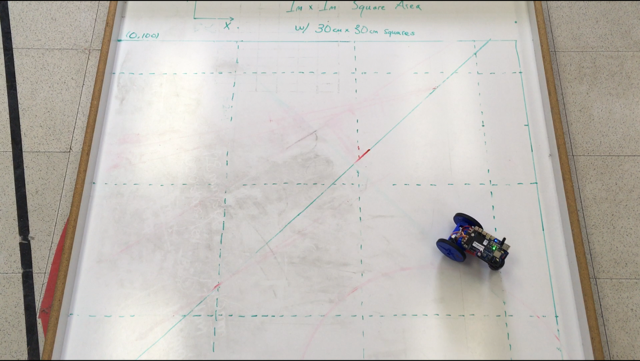
\includegraphics[width=0.38\textwidth]{figs/img/lineFollowerAt2.PNG}
    }\\
    \subfigure[][]{
    \label{fig:trajectoryLineFollowerPic2}
    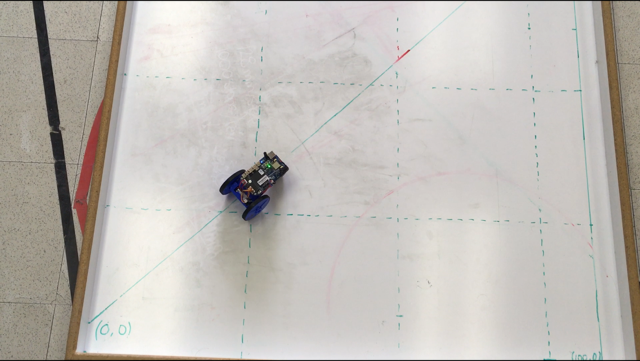
\includegraphics[width=0.38\textwidth]{figs/img/lineFollowerAt7.PNG}
    }    
    %\includegraphics{}
    \caption{MAFOSS running line--following algorithm using an eduMOD differential drive mobile robot.}
    \label{fig:trajectoryLineFollowerPictures}
\end{figure}
%
The corresponding robot trajectory is plotted in Fig.~\ref{fig:trajectoryLineFollower}. Fig.~\ref{fig:errorLineFollower} shows the orthogonal distance between the robot and the line. Note that the purpose here is to demonstrate different mobile robot/agent based navigation algorithms using the MAFOSS. 
\begin{figure}
    \centering
    \subfigure[][]{
    \label{fig:trajectoryLineFollower}
    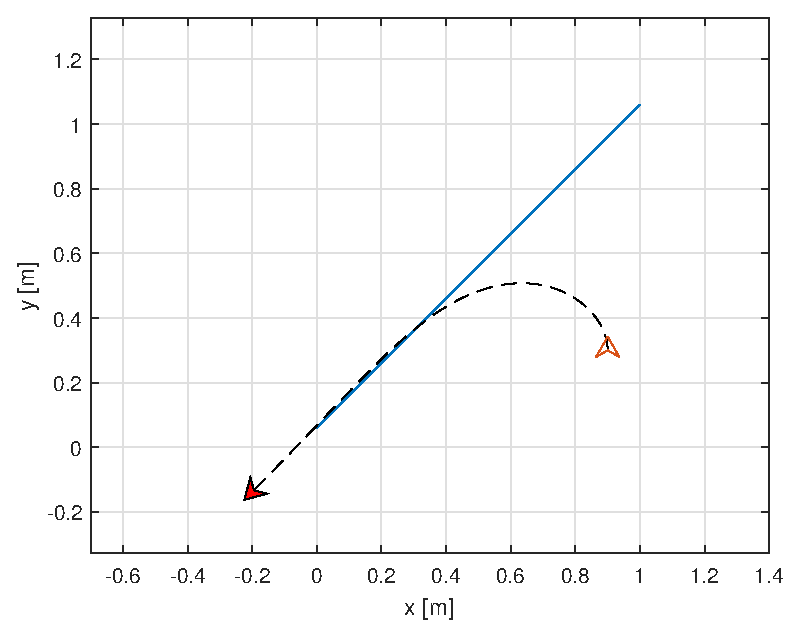
\includegraphics[width=0.36\textwidth]{figs/matlab/lineFollower/trajectory.eps}
    }\\
    \subfigure[][]{
    \label{fig:errorLineFollower}
    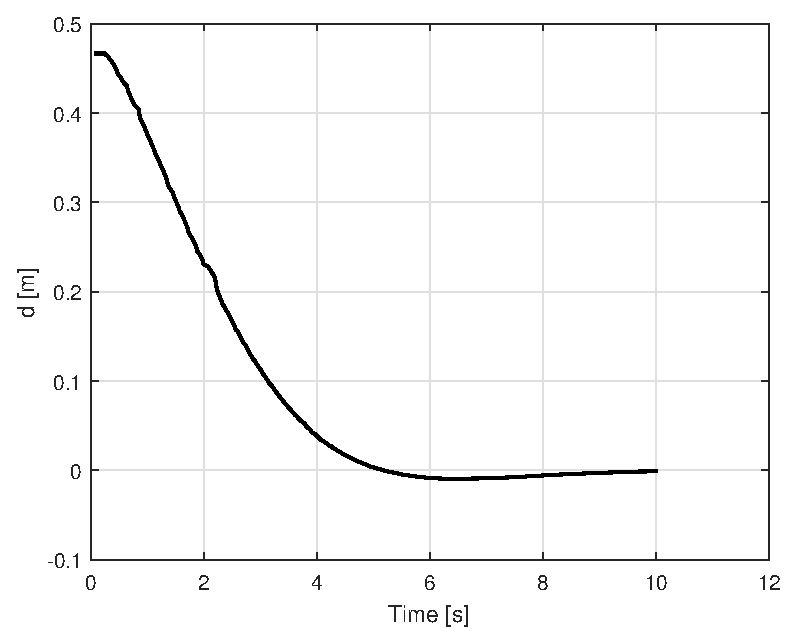
\includegraphics[width=0.36\textwidth]{figs/matlab/lineFollower/error.eps}
    }
    \caption{Performance of MAFOSS in running leader--follower algorithm.}
    \label{fig:performanceLineFollower}
\end{figure}


\subsection{Leader Follower}
The aim of this section is to further evaluate the MAFOSS by running a relatively complex scenario, such as the leader--follower problem, using two EduMOD robots. In this scenario, the leader attempts to follow a circular trajectory and the follower attempts follow behind the leader. The radius of the target circle was set to be $32~[\centi\meter]$, its center was set to $(0,0)~\si{\meter}$, and the desired distance offset between the leader and follower was $15~[\centi\meter].$ The leader was initially placed at $(x,y) = (0.1, -0.2)~\si{\meter}$ with an orientation of $\theta = 0$ while the follower was initially placed at $(x,y) = (-0.2, -0.2)~\si{\meter}$ with an orientation of $\theta = 0$ %% 
\begin{figure}
    \centering
    \subfigure[][]{
    \label{fig:trajectoryLeaderFollowerPic1}
    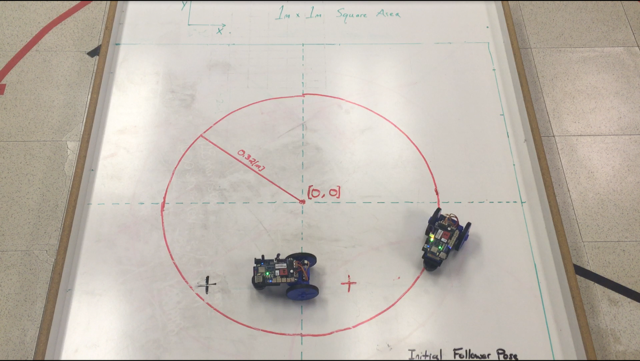
\includegraphics[width=0.42\textwidth]{figs/img/leaderFollowerAt5.PNG}
    }\\
    \subfigure[][]{
    \label{fig:trajectoryLeaderFollowerPic2}
    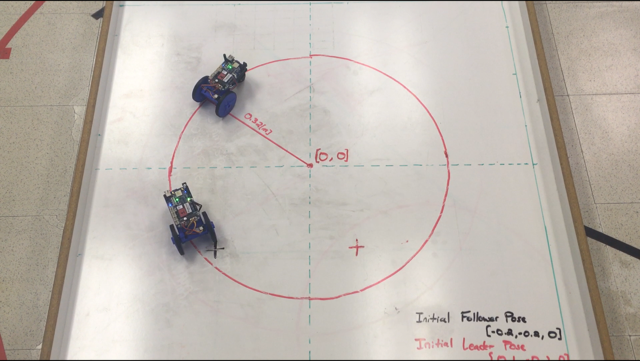
\includegraphics[width=0.42\textwidth]{figs/img/leaderFollowerAt60.PNG}
    }    
    %\includegraphics{}
    \caption{MAFOSS running leader--follower algorithm using two eduMOD differential drive mobile robots.}
    \label{fig:trajectoryLeaderFollowerPictures}
\end{figure}
%
follow a leader robot that navigates along a circular path defined by %
%
\begin{subequations}
  \label{eq:refTrajectory}
\begin{align}
  x^{[d]}(t) &= x_c + R\cos(\alpha t)\\
  y^{[d]}(t) &= y_c + R\sin(\alpha t), 
\end{align}  
\end{subequations}

%
where $(x_c,y_c)$ is the coordinate of the center of the circular path with radius $R>0,$ $\alpha$ is the angular rate parameter of the circle at time $t\ge 0.$ The tangent of the trajectory~\eqref{eq:refTrajectory} gives the angle $\theta^{[d]}(t),$ which is computed as $\theta^{[d]}(t) = \mathrm{atan2}(\dot y^{[d]},\dot x^{[d]}).$  The  linear and angular speeds of the leader robot are given by %
%
% \begin{subequations}
\begin{align*}
  \nu^{[d]} = \sqrt{(\dot x^{[d]})^2 + (\dot y^{[d]})^2}~~\text{and}~~
  \omega^{[d]}  = \frac{\ddot y^{[d]} \dot x^{[d]}-\ddot x^{[d]} \dot y^{[d]}}{(\nu^{[d]})^2}.
\end{align*}
% \end{subequations}
%
The follower robot can be  modeled as a unicycle with its kinematics given in~\eqref{eq:unicycleModel}. The problem is to find the linear and angular speeds, $\nu(t)$ and $\omega(t),$ of the follower robot so that it follows the leader robot that follows the reference trajectory~\eqref{eq:refTrajectory} while maintaining a constant geometric distance. %  
%
\begin{figure}
    \centering
    \subfigure[][]{
    \label{fig:trajectoryLeaderFollower}
    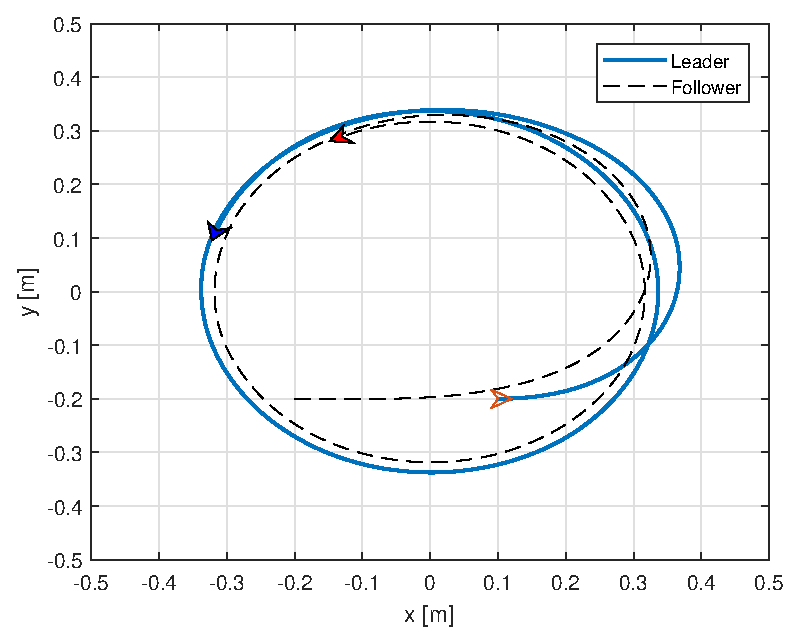
\includegraphics[width=0.48\textwidth]{figs/matlab/leaderFollower/trajectory.eps}
    }\\
    \subfigure[][]{
    \label{fig:errorLeaderFollower}
    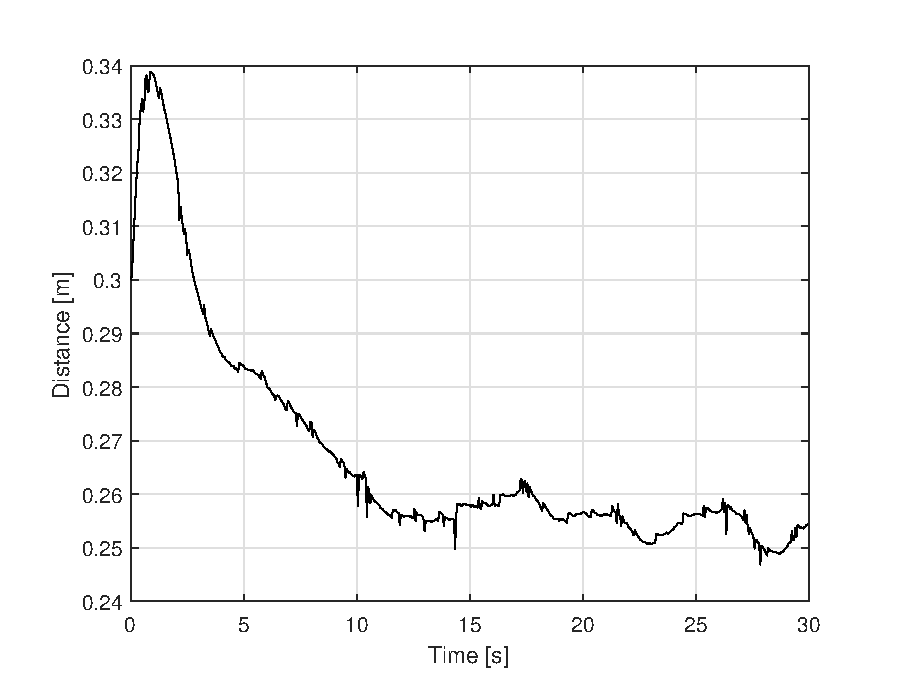
\includegraphics[width=0.52\textwidth]{figs/matlab/leaderFollower/leaderFollowerImplementDistance.eps}
    }
    \caption{Performance of MAFOSS in running leader--follower algorithm.}
    \label{fig:performanceLeaderFollower}
\end{figure}
%
For the robot to follow the circular path, let us define the position error
%
\begin{align*}
    e(t) = \sqrt{(x^{[d]}(t) - x(t))^2+(y^{[d]}(t) - y(t))^2} - d_{\text{offset}}
\end{align*} 
%
with $d_{\text{offset}}$ being the distance that the robot supposed to maintain from the desired position $(x^{[d]}(t),y^{[d]}(t)).$ The robot's linear speed to follow the path is given by  
%
\begin{align*}
  \nu(t) = K_ve(t) + K_i\int_0^t[e(t)]\mathrm{dt},
\end{align*}
%
where $K_v, K_i>0$ are constant proportional gains. The robot is directed to steer towards the circle with a steering angle given by%
%
%\begin{align*}
  $\gamma = K_\gamma \tilde\theta,$ %
%\end{align*}
%
where $\tilde\theta = (\theta^{'} - \theta)$ with $\theta^{'} = \mathrm{atan2}(y^{[d]}-y,x^{[d]}-x)$ and the proportional gain $K_\gamma>0.$ Note that the angular difference $\tilde\theta\in (-\pi,\pi].$ The values of the parameters used in this experiment are $K_v = 0.35,~K_i = 0$ and $K_\gamma = 0.45.$ The performance of MAFOSS in running a simple leader--follower algorithm is demonstrated in Fig.~\ref{fig:trajectoryLeaderFollowerPictures}, where the follower is following the leader robot on the circular path. The X-Y trajectories of these robots and their distance are shown in Fig.~\ref{fig:performanceLeaderFollower}. As can be seen, the proposed MAFOSS has the ability to run multi-agent algorithms with various complexities. 




\section{Conclusion}
\label{sec:conclusion}
In this paper, we have presented a new framework, MAFOSS, that can be used to implement algorithms for multi-agent systems. Two different experiments have been conducted to show the proposed framework's ability to conduct motion control algorithms using multiple differential drive mobile robots/agents. A potential future work will include testing the proposed MAFOSS for implementing more complex multi-agent control algorithms, such as area coverage control and cooperative estimation while incorporating sensory measurements. 



%%% Local Variables:
%%% mode: latex
%%% TeX-master: "../finalReportMainV1"
%%% End:

%======================================================================
\chapter{Computer Simulations using V-REP}
\label{chap:VREP}
%======================================================================

%======================================================================
\chapter{Experimental Validation using MAFOSS}
\label{chap:experimentalResults}
%======================================================================

%======================================================================
\chapter{Conclusion and Future Work}
\label{chap:conclusion}
%======================================================================


% %----------------------------------------------------------------------
% % APPENDICES
% %---------------------------------------------------------------------- 
% \appendix
% % Designate with \appendix declaration which just changes numbering style 
% % from here on
% % Add a title page before the appendices and a line in the Table of Contents
% \chapter*{APPENDICES}
% \addcontentsline{toc}{chapter}{APPENDICES} 
% %
% % An appendix
%======================================================================
\chapter{Sources of Information and Help}
\label{ch:Appendix-Sources-of-Info}
%======================================================================
The best source of information about \LaTeX\ is the two books mentioned in this course \cite{lamport.book,goossens.book}.
Another excellent resource is the UseNet newsgroup \verb=comp.text.tex=.
A frequently-asked-questions (FAQ) list is also maintained by this news group.
You might also search the World Wide Web for ``LaTeX'' for other sources of help.


%%% Local Variables:
%%% mode: latex
%%% TeX-master: "../finalReportMainV1"
%%% End:
 %"Sources of Information and Help"
% % An appendix
%======================================================================
\chapter[PDF Plots From Matlab]{Matlab Code for Making a PDF Plot}
\label{ch:Appendix-Matlab} 
%======================================================================
\section{Using the GUI}
Properties of Matab plots can be adjusted from the plot window via a graphical interface. Under the Desktop menu in the Figure window, select the Property Editor. You may also want to check the Plot Browser and Figure Palette for more tools. To adjust properties of the axes, look under the Edit menu and select Axes Properties.

To set the figure size and to save as PDF or other file formats, click the Export Setup button in the figure Property Editor.

\section{From the Command Line} 
All figure properties can also be manipulated from the command line. Here's an example: 
\begin{verbatim}
x=[0:0.1:pi];
hold on % Plot multiple traces on one figure
plot(x,sin(x))
plot(x,cos(x),'--r')
plot(x,tan(x),'.-g')
title('Some Trig Functions Over 0 to \pi') % Note LaTeX markup!
legend('{\it sin}(x)','{\it cos}(x)','{\it tan}(x)')
hold off
set(gca,'Ylim',[-3 3]) % Adjust Y limits of "current axes"
set(gcf,'Units','inches') % Set figure size units of "current figure"
set(gcf,'Position',[0,0,6,4]) % Set figure width (6 in.) and height (4 in.)
cd n:\thesis\plots % Select where to save
print -dpdf plot.pdf % Save as PDF
\end{verbatim} 


%%% Local Variables:
%%% mode: latex
%%% TeX-master: "../finalReportMainV1"
%%% End:
 %"Matlab Code for Making a PDF Plot"

% %----------------------------------------------------------------------
% % END MATERIAL
% %----------------------------------------------------------------------

% % B I B L I O G R A P H Y
% % -----------------------
% %
% The following statement selects the style to use for references.  It controls the sort order of the entries in the bibliography and also the formatting for the in-text labels.
\bibliographystyle{plain}
% This specifies the location of the file containing the bibliographic information.  
% It assumes you're using BibTeX (if not, why not?).
\ifthenelse{\boolean{PrintVersion}}{
\cleardoublepage % This is needed if the book class is used, to place the anchor in the correct page,
                 % because the bibliography will start on its own page.
}{
\clearpage       % Use \clearpage instead if the document class uses the "oneside" argument
}
\phantomsection  % With hyperref package, enables hyperlinking from the table of contents to bibliography                        
% % The following statement causes the title "References" to be used for the bibliography section:
% % \renewcommand*{\bibname}{References}
% Bibliography 
\renewcommand{\bibname}{Bibliography}

% Add the References to the Table of Contents
\addcontentsline{toc}{chapter}{\textbf{References}}

\bibliography{bib/refsMultiAgent,bib/seniorProject2-2018,bib/refsSuruzWeb,bib/refsBooksTRTheses}
% Tip 5: You can create multiple .bib files to organize your references. 
% Just list them all in the \bibliogaphy command, separated by commas (no spaces).


%----------------------------------------------------------------------
\end{document}
%======================================================================



%%% Local Variables: 
%%% mode: latex
%%% TeX-master: t
%%% End: 
